\documentclass[12pt,oneside]{report}
\usepackage{latexsym}
%\usepackage{auto-pst-pdf}
\usepackage{pstricks}
\usepackage{epsf}
\usepackage{epstopdf}
\usepackage{epsfig}
\usepackage{graphicx}
\usepackage{a4wide}
\usepackage{amsmath}
%\usepackage{ifsym}
%\usepackage[chapter]{algorithm}
%\usepackage{algorithmic}
\usepackage{amssymb}
\usepackage{graphicx}
\usepackage{multirow}
\usepackage{float}
\usepackage{subfig}
\usepackage{cite}
\usepackage{url}
%\usepackage{hyperref}
\usepackage[linktocpage=true]{hyperref}
%[pdftex]{graphicx} %For pdflatex command
%\usepackage[dvips]{graphics} %For latex command
\parskip 5pt

\def\head#1{{\medskip \bf \noindent #1}}
\def\binom#1#2{{#1 \choose #2}}
\def\ilh#1{\vspace{0.1in}\noindent {\bf #1}}
\def\str#1#2{{#1}_1{#1}_2\dots{#1}_{#2}}
\def\strg#1#2#3{{#1}_{#2}\dots{#1}_{#3}}
\def\seq#1#2{{#1}_1,{#1}_2,\dots,{#1}_{#2}}
\def\v#1{$#1$}
\def\msf#1{\mbox{\it #1}}
\newtheorem{thm}{Theorem}[chapter]
\newtheorem{lem}[thm]{Lemma}
\newtheorem{defn}[thm]{Definition}
\newtheorem{cor}[thm]{Corollary}

\newcommand\INPUT{\item[\textbf{Input:}]}
\newcommand\OUTPUT{\item[\textbf{Output:}]}
\newcommand\BEGIN{\item[\textbf{begin}]}
\newcommand\END{\item[\textbf{end}]}

\newcommand\qed{\hfill{\ensuremath{\Box}}\par\addvspace{\topsep}}
\newenvironment{proof}{\begin{trivlist}
	\item[\hskip\labelsep{\bfseries Proof:}]}{\hfill$\Box$\end{trivlist}}
\newenvironment{claim}{\begin{trivlist}
	\item[\hskip\labelsep{\bfseries Claim:}]\itshape}{\end{trivlist}}

\newcommand{\picx}[2]{\setlength{\epsfxsize}{#2}\mbox{\epsffile{#1}}}
\newcommand{\pica}[2]{\setlength{\epsfxsize}{#2}\mbox{\epsffile{#1}},angle=270}
\newcommand{\picy}[2]{\setlength{\epsfysize}{#2}\mbox{\epsffile{#1}}}
\newcommand{\picr}[1]{\mbox{\epsffile{#1}}}
\renewcommand{\baselinestretch}{1}
% 
% \newfont{\iitblogofont}{iitblogo} 
% \newcommand{\iitbseal}{{\iitblogofont a}}
% \renewcommand{\bibname}{References}
% \newlength{\logowidth}
% \settowidth{\logowidth}{\iitbseal}

% the document begins here ----------------------------------------------
\begin{document}

% the title page ----------------------------------------------------------
\pagestyle{empty}
\begin{center}
{\Large Ph.D. Annual Progress Report}

\vspace{1cm}

{\LARGE \bf Low Power Level Crossing A to D Converter} 
 
\vspace{2.0cm}

by

\vspace{0.5cm}

{\Large \bf Janamani C. Ayyangalam}

\vspace{0.25cm}

08407604

\vspace{1.5cm}

Under the guidance of

\vspace{0.5cm}

{\Large \bf Prof. A. N. Chandorkar}


\begin{figure}[h]
\hspace{1cm}
\vspace{1cm}
\begin{center}
\includegraphics[scale=0.75]{./Figures/IITBombayLogo.ps}
\end{center}
\vspace{1cm}
\end{figure}

Department  of Electrical Engineering \\
\vspace{0.25cm}
Indian Institute of Technology, Bombay\\
\vspace{0.25cm}
April 2015 \\
\vspace {0.5cm}

\end{center}
%\pagebreak

%-------------------------abstract---------------------------------
\begin{center}
\abstract
\end{center}

\par
\hspace{0.5cm} Due to the increasing importance of products like laptops, music players, cell phones and implantable bio-medical products which are operated using batteries, it has became imperative to prolong the battery life as much as possible to achieve high performance. No significant improvements have been made in the energy density of commonly available batteries from many years. All batteries are limited to a maximum amount of energy per unit volume. The bigger the battery compartment, the longer the battery will last. On the other hand, advancements in CMOS technology is much faster than compared to the advancements in battery technology. By doubling the number of transistors on a chip for every two years, the battery technology is not sufficient to provide required power for the chips to attain an optimum performance. Hence, power reduction is an important and challenging target for these type of products.

\par
\hspace{0.5cm} Generally most of the real time signals are in analog form, for example sound generated vocally from human beings, bio-medical signals like electroencephalograph, electrocardiograph. Also, human beings perceive and retain information in analog form. Analog processing of these signals is very difficult because of the noise interference. Hence, Digital Signal Processing is used to process these signals because they are less prone to noise interference and advanced Digital Signal Processing algorithms made signal processing easy in digital domain. So, to convert these analog signals into digital signals analog-to-digital converters are used and similarly digital-to-analog converters are used to convert digital signals into analog signals for further processing. Systems like bio-chips which are implanted in the human body should consume very less power, at the same time we have to maintain its performance. Hence, it is quite challenging to come up with a low power and high speed analog-to-digital and digital-to-analog converters. In both these converters resolution, speed and power consumptions are most important features.

\par
\hspace{0.5cm} Importance of battery run systems continues to grow day by day. Traditional approaches to designing these systems vary from typical semiconductor design. Every low power design is different and will have its own interesting set of problems to solve. We have to think through every element of the design if we want to operate at low power levels. Some of important issues are to consider include power consumption limits, speed and size restrictions. Speed is one of the most important problem in low power design. Increase in speed results in higher power consumption. Similarly increase in area of the chip also results increase in power consumption. In this work an attempt has been made to design an analog-to-digital converter which consumes low power in applications where the signal should be monitored continuously and vary brief amount of time like pressure controller and flow controls etc.
 
%------------------------------------------------------------------

%-------------------------content----------------------------------
\evensidemargin -0.25in
\newpage
\pagenumbering{roman}
\tableofcontents
\listoffigures
%\listoftables
\clearpage
\pagenumbering{arabic}
%------------------------------------------------------------------



\newtheorem{definition}{Definition}[chapter]
\newtheorem{example}{Example}[chapter]

% to get the name of the chapter on top of the pages
\pagestyle{plain}

\chapter{Introduction}

\par
\hspace{1.2cm} Most of the systems using analog-to-digital converters (ADC's) bring signals with interesting statistical properties into operation, but Nyquist signal processing architectures do not take advantage of these properties. Actually, these signals (such as temperature sensors, pressure sensors, electro-cardiograms etc.) are almost always constant and may vary significantly only during brief moments like electrocardiograph as shown in Fig.~\ref{fig:ECG}. 

\begin{figure}[H]
	\begin{center}
		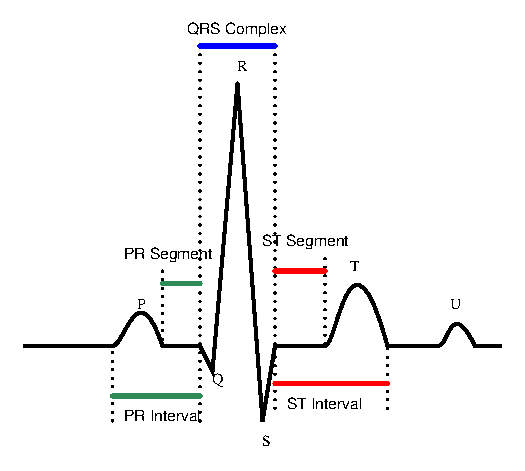
\includegraphics[scale=0.80]{./Figures/ECG.ps}
		\caption{Electrocardiograph (ECG) Signal.}
		\label{fig:ECG}
	\end{center}
\end{figure}

\par
\hspace{0.6cm} The classical regular sampling and converting systems are highly constrained, due to the Shannon theory, which is to ensure for the sampling frequency to be at least twice the maximum input signal frequency. Therefore, in the time domain, this condition can be translated as a large number of samples without any relevant information. This effect implies a useless increase of activity of the circuit compared to the supplied output digital information relevance, and so a useless increase of the power dissipation. It has been proved that ADC's using a non equi-repartition of the samples in time lead to interesting power savings compared to Nyquist ADC's~\cite{1522735}.



\section{Level cross sampling scheme}

\par
\hspace{0.6cm} The principle of level crossing ADC's is the dual case of Nyquist ADC's. In Nyquist \mbox{ADC's} the samples are taken at fixed intervals of time with reference to the clock signal. The minimum clock signal is chosen to be twice the maximum frequency of the analog input signal. For signals in which the frequency content is very low for most of the time, with rare occurrences of high frequency contents, it leads to over sampling. Hence, taking samples at regular intervals of time unnecessarily increases circuit activity, which in turn increases the power consumption~\cite{sayiner1996level}. 

\begin{figure}[H]
	\begin{center}
		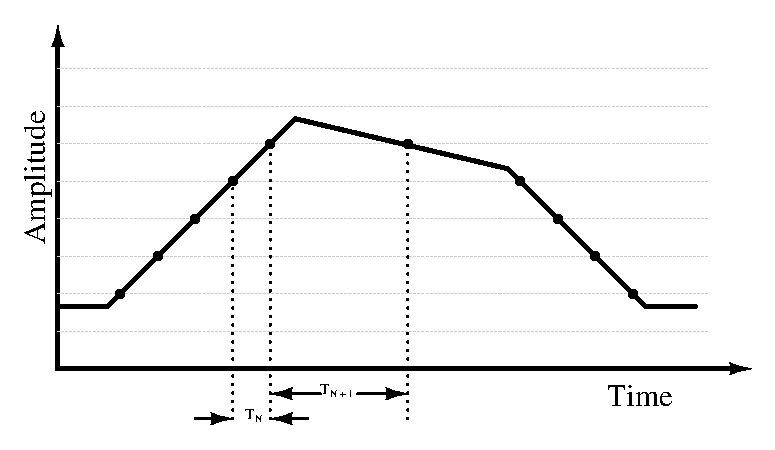
\includegraphics[scale=0.75]{./Figures/LCS.ps}
		\caption{Principle of the level cross sampling scheme. }
		\label{fig:LCS}
	\end{center}
\end{figure}

\par
\hspace{1.2cm} In Nyquist ADC's the time instants are perfectly known and samples of amplitude are quantized, where as in case of level crossing ADC's the amplitude levels are known and the samples of time are quantized. Fig.~\ref{fig:LCS} shows the level cross sampling scheme~\cite{1595684}. In level crossing ADC's the occurrence of samples depend on signal amplitude variations, this sampling scheme removes the conversion of redundant samples or samples without any relevant information when the analog signal is quiet. Therefore, it leads to a compression of digital samples and reduction in the activity of the circuit. Level cross sampling is best suited for asynchronous and low power applications~\cite{allier2003new}. Difference between Nyquist sampling and level cross sampling schemes is illustrated in Table.~\ref{tab:DNL}. 

\begin{table}[H]
	\caption{Difference Between Nyquist \& Level Cross Sampling Schemes}
	\label{tab:DNL}
	\begin{center}
	\resizebox{10cm}{!}{
		\begin{tabular}{c|c|c|}
			\cline {2-3} %\hline
		 	&{Nyquist Sampling} & {Level Cross Sampling} \\ \hline
			\multicolumn {1}{|c|} {Conversion Trigger} 	&  {Clock} 			&  {Level Crossing} 	\\ \hline
			\multicolumn {1}{|c|} {Amplitude} 			&  {Quantized} 		&  {Exact Value} 		\\ \hline
			\multicolumn {1}{|c|} {Time} 				&  {Exact Value} 	&  {Quantized} 			\\ \hline
			\multicolumn {1}{|c|} {SNR Dependency} 		&  {Number of Bits} &  {Timer Period} 		\\ \hline
			\multicolumn {1}{|c|} {Converter Output} 	&  {Amplitude} 		&  {Amplitude \& Time} 	\\ \hline
		\end{tabular} }	
	\end{center}
\end{table}

\par
\hspace{0.6cm} In level crossing ADC's for M-bits resolution it requires $2^M-1$ quantization levels are regularly disposed along the amplitude range of the input signal $V_{in}$. A sample is taken only when the analog input signal $V_{in}$ crosses one of quantization levels. Contrary to classical Nyquist sampling, samples are not regularly spaced out in time, because it depends on the variation of input signal $V_{in}$~\cite{allier2005asynchronous}.

\begin{figure}[H]
	\begin{center}
		\includegraphics[height=10 cm, angle=270]{./Figures/ECGS.ps}
		\caption{Level cross sampling scheme for an ECG signal}
		\label{fig:ECGS}
	\end{center}
\end{figure}

\par
\hspace{0.6cm} 	The level cross sampling scheme can be understood by using Fig.~\ref{fig:ECGS}, which shows a typical ECG signal. Level crossing \mbox{ADC's} are driven by the level cross rather than by clock ie., the conversion process triggers when the analog input crosses any of the quantization levels. The dotted lines represent quantization levels. The shape of the analog input signal can be preserved by calculating the time difference between two successive samples. Thus, outputs from level crossing \mbox{ADC's} are amplitude and time data pairs, unlike that of Nyquist \mbox{ADC's} where the output consists of only amplitude data. 




\par
\hspace{0.6cm} The time taken from analog input crossing one of the quantization levels to complete conversion process is called loop delay of that level crossing ADC. The loop delay of the level crossing ADC's decides the maximum input signal frequency which can be track without slope overload error by the level crossing ADC. Fig.~\ref{fig:SOE} shows slope overloading error in level crossing ADC. The maximum frequency of the input with which the level crossing ADC can track without slope overload error can be calculated by using loop delay of the level crossing ADC~\cite{allier2005120nm}.



\par
\hspace{0.6cm} There are some drawbacks in level cross sampling ADC's, timer will define the resolution of the level crossing ADC's, which requires separate high speed clock generation circuit for timer to calculate the difference between present sample and previous sample. When tracking analog input signal it follows linear successive approximation which can't track sharp raise and fall edges in analog input signal~\cite{5672382}. When designing level crossing ADC's one must know the statistical properties of the signal clearly, once designed for particular application it can't be used for other application effectively. 

\begin{figure}[H]
	\begin{center}
		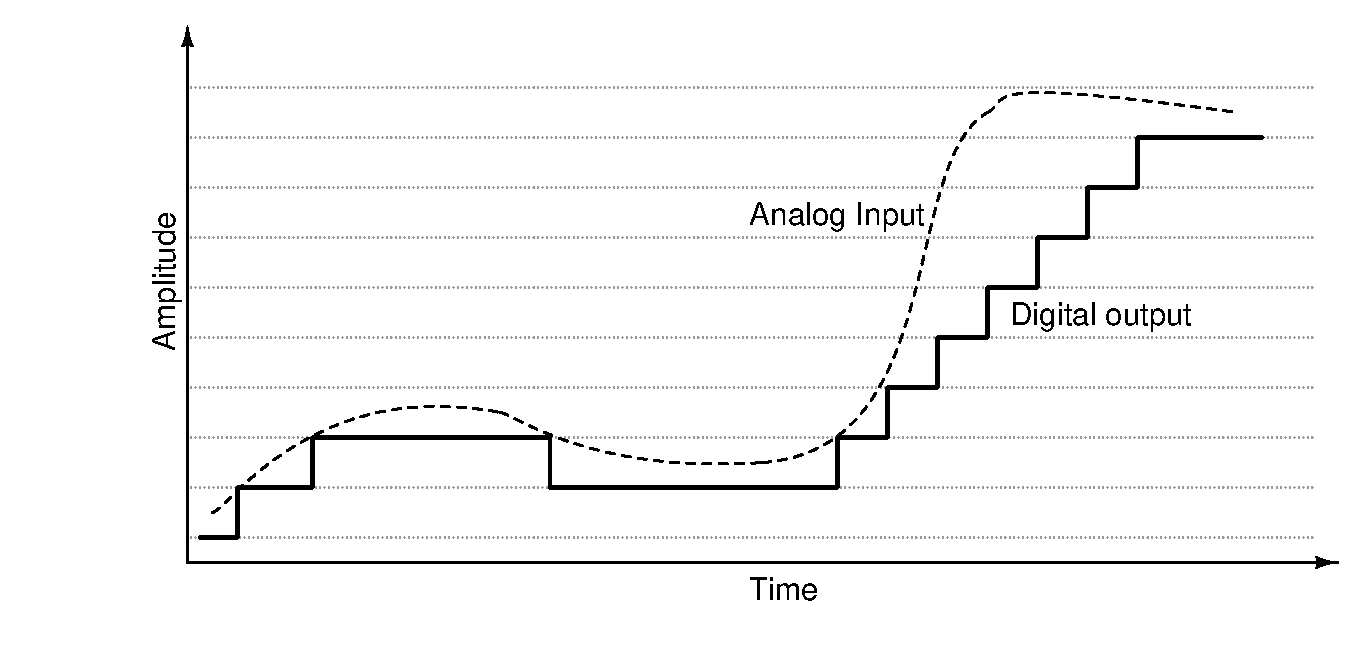
\includegraphics[scale=0.5]{./Figures/SOE.ps}
		\caption{Slope overloading error in LC-ADC}
		\label{fig:SOE}
	\end{center}
\end{figure}

\par
\hspace{0.6cm} The proposed architecture is aimed to reduce this loop delay so that it can track high frequency components in input analog signal without slope overloading error. It is achieved by reducing the conversion steps when the signal changes rapidly by checking for complete analog input range by incorporating binary search algoritham in conversion process.


\section{Organization of the Report}

\par
\hspace{1.2cm} The remainder of the report is organized as follows. Chapter 2 gives a brief overview on literature review of the level crossing ADC architectures. Chapter 3 describes the  proposed ADC architectures, its principle is based on a level cross sampling scheme that allow reduction in activity of the circuit. Chapter 4 presents building blocks and simulation results. Chapter 5 describes conclusion and future work.




\chapter{Literature Review}
	
\par
\hspace{0.6cm} Most of the reported level crossing ADC's suffer from the large loop delay which results in slope overloading error. Some of the authors tried to eliminate the slope overload problem in level crossing ADC's, but they end up in increasing complexity or with some other problem. Following section breifly describes the attempts made to eliminate the slope overload problem in level crossing ADC's.


\section{ Level crossing ADC}

\par
\hspace{0.6cm} Level cross sampling is best suited for asynchronous ADC's. Fig.~\ref{fig:REFA} shows a block diagram of level crossing ADC architecture~\cite{4672051}. The architecture of the level crossing ADC is a tracking loop controlled by the analog input signal $V_{in}$. It is composed of a difference quantificator, an up/down counter, a digital-to-analog converter (DAC), and a timer. Difference quantificator behaves like a window detector, when the analog input $V_{in}$ is with in the specified range both outputs $INC$ and $DCR$ from difference quantificator are zero. 

\begin{figure}[h]
	\begin{center}
		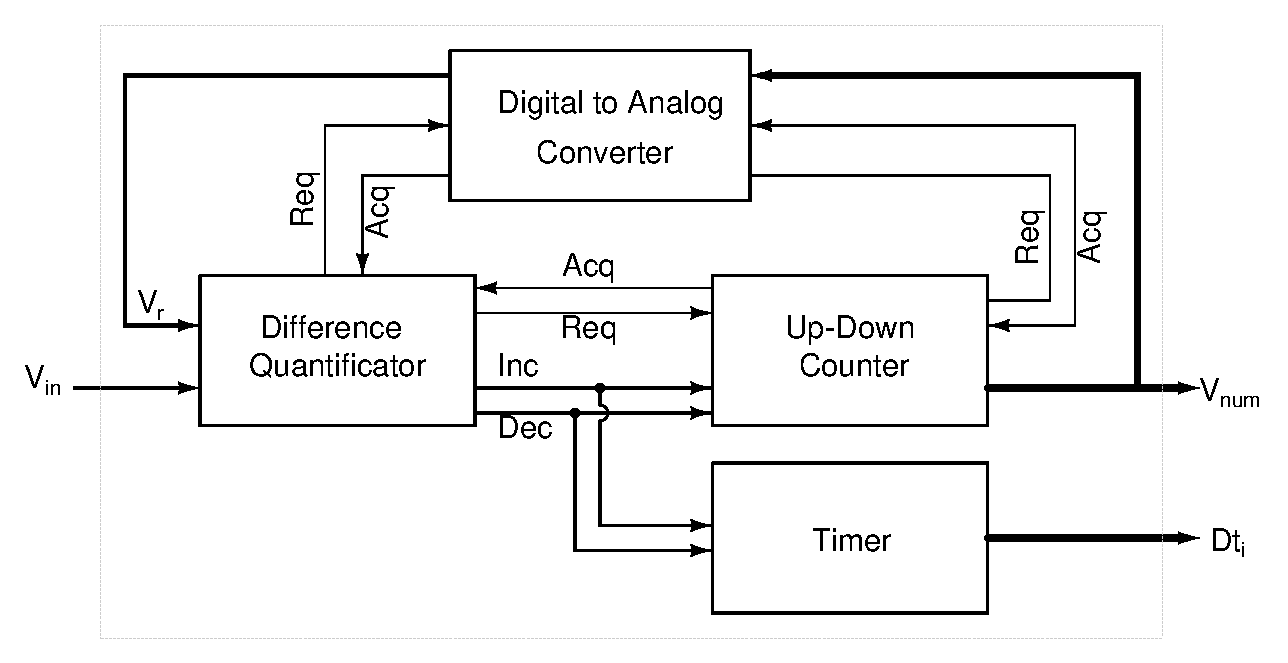
\includegraphics[scale=0.45]{./Figures/REFA.ps}
		\caption{Block Diagram of level crossing ADC.}
		\label{fig:REFA}
	\end{center}
\end{figure}

\par
\hspace{0.6cm}If the analog input $V_{in}$ crosses the specified range it generates either $INC$ or $DCR$ depending on the direction of analog input $V_{in}$. Generally the range of the difference quantificator will be +LSB to -LSB of the reference signal generated by the DAC. Up/down counter counts the number of transitions the analog input $V_{in}$ have. If the $INC$ signal from difference quantificator becomes '1' the counter contents will be incremented by one, if the $DCR$ signal generated from difference quantificator becomes '1' the contents of the counter are decremented by one, in a simplified sense the contents of the up/down counter refers to the digital value corresponding to then analog input value of the level crossing ADC. 

\par
\hspace{0.6cm} The DAC which converts the digital input form  up/down counter in to the corresponding analog value, which is used to generate the reference value for the difference quantificator. Timer is driven by high speed clock which counts the time difference between the present sample and the previous sample. All the hand shaking signals are asynchronous between the block. Once the whole operation is completed it waits till another transition occurred in the difference quantificator. 

\par
\hspace{0.6cm} 	Generally the up-down counter in level crossing ADC is implemented using an adder-subtractor circuit. As the number of bits in up-down counter increases the delay in calculating the up-down counter value increases when a trigger generated by the difference quantificator. This increase in delay results in increased loop delay of the level crossing ADC. If the loop delay of the  level crossing ADC increases, it effectively reduces the maximum frequencies in the input signal which it can track without slope overload error. 




\section{ Signal-dependent variable-resolution ADC}


\par
\hspace{0.6cm} The authors kurchuk et al have suggested signal dependent variable resolution quantization technique to reduce slope overload error. Fig.~\ref{fig:REFB} shows a block diagram of slope dependent variable resolution quantization level crossing ADC architecture~\cite{kurchuk2009signal}. In this technique a slope detector at the input of ADC is used to measure the slope of the input analog signal. Depending on the slope of the input analog signal, the controller circuit in level crossing ADC changes the resolution of the level crossing ADC. 

\begin{figure}[h]
	\begin{center}
		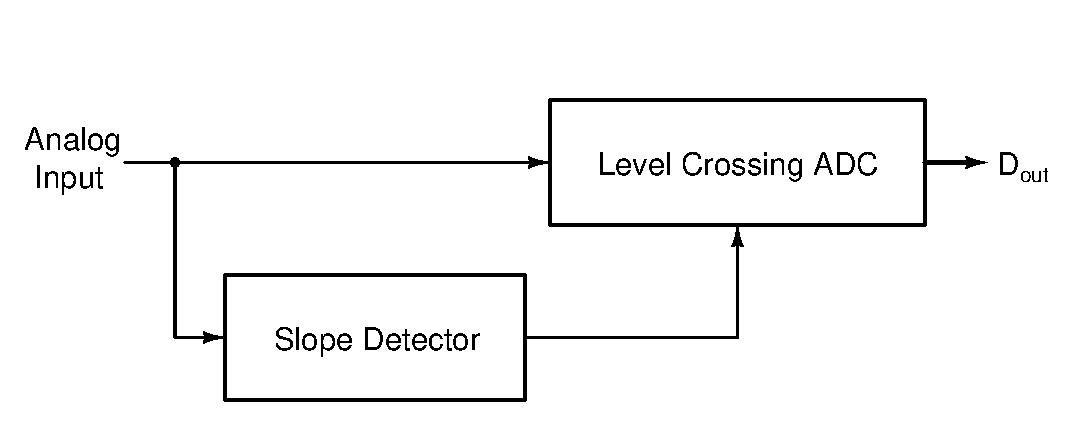
\includegraphics[scale=0.6]{./Figures/REFB.ps}
		\caption{Block Diagram of level crossing ADC.}
		\label{fig:REFB}
	\end{center}
\end{figure}

\par
\hspace{0.6cm} The effectiveness of this technique depends on how accurately the slope is measured by the input slope detector. In this technique the complexity of the level crossing ADC increases with the number of bits to represent the slope. There is some delay in the output because first the slope detector should detect the the slope then the conversion process is started.






\section{ Adaptive asynchronous ADC}

\par
\hspace{0.6cm} The authors Agarwal et al have suggested Adaptive asynchronous technique to reduce slope overload error. As the up-down counter linear fasion the autors replaced the up-down counter with the logic shown in Fig.~\ref{fig:REFC} in variable input slope dependent level crossing ADC architecture~\cite{agarwal2009adaptive}. The PSL block in block diagram is a pulse stretching logic, which is implemented with the low pass R-C filter. When any of the outputs of difference quantificator are high these PSL blocks extenend the pulse duration of the outputs of difference quantificator and the delay elements store it's value. Depending on the outputs of delay elements and outputs of the difference quantificator the increment/decrement step size is changed in controller logic. In this technique previous bits are stored, based on which the slope is estimated and the resolution of level crossing ADC is adjusted. 

\begin{figure}[h]
	\begin{center}
		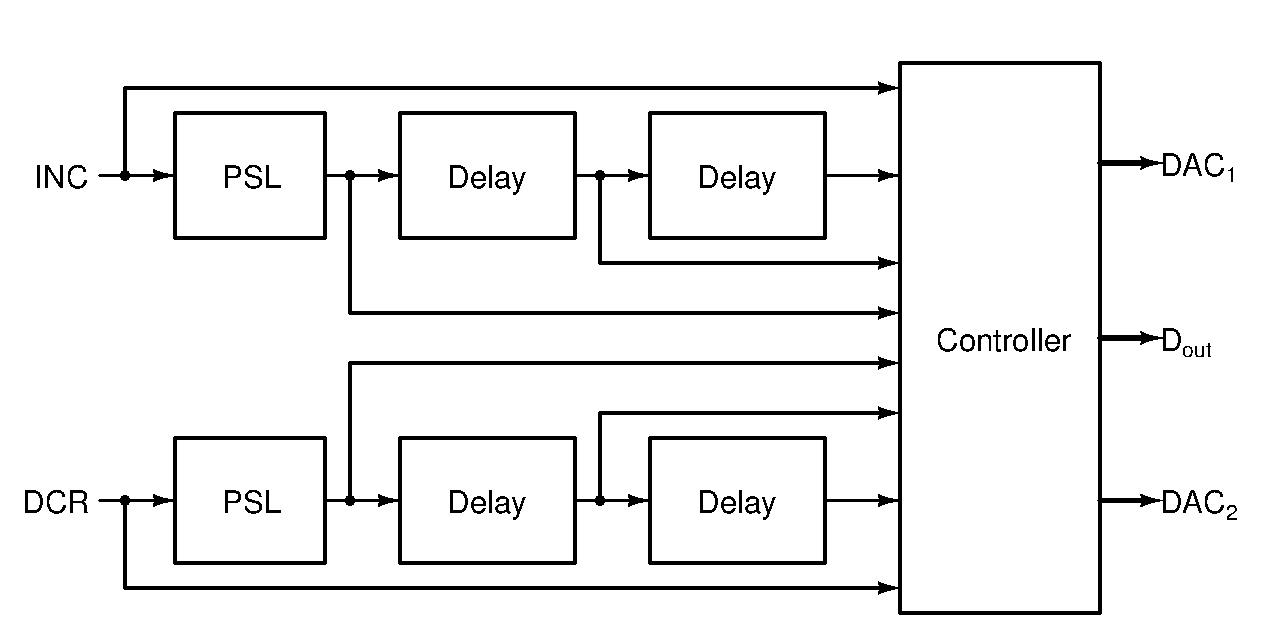
\includegraphics[scale=0.45]{./Figures/REFC.ps}
		\caption{Block Diagram of level crossing ADC.}
		\label{fig:REFC}
	\end{center}
\end{figure}

\par
\hspace{0.6cm} This technique has significant chances of misinterpreting the output when the slope of the input signal is changing. Apart from misinterpretation, the complexity of the circuit is proportional to the number of bits used to set its resolution.



 
\par
\hspace{0.6cm} The proposed architecture solves slope overloading error problem with minimal increase in complexity. The proposed technique is purely deterministic. In addition to improved performance, the proposed architecture can be reconfigured to operate in Nyquist mode. The proposed architecture also reduces power consumption when operated in Nyquist mode as compared to conventional successive approximation ADC's by reducing number of comparisions.




















\chapter{Proposed ADC Architecture}

\par
\hspace{1.2cm} The proposed architecture works based on level cross sampling scheme. Fig.~\ref{fig:PADC} shows the block diagram of the proposed ADC. Intially the sample and hold (SAH) is in sampling mode, the DAC in successive approximation ADC generates the refernce signals needed for the difference quantificator. Varition in the input analog signal crosses any of the refernce signals generated by the DAC in successive approximation ADC then difference quantificator generates conversion signal to the controller circuit and the controller circuit placeses the SAH circuit in hold mode until the conversion process is completed. Otherwise, the SAH is in sampling mode until the input anlog signal crosses any of the refence signal generated by DAC in successive approximation ADC. 

\begin{figure}[h]
	\begin{center}
		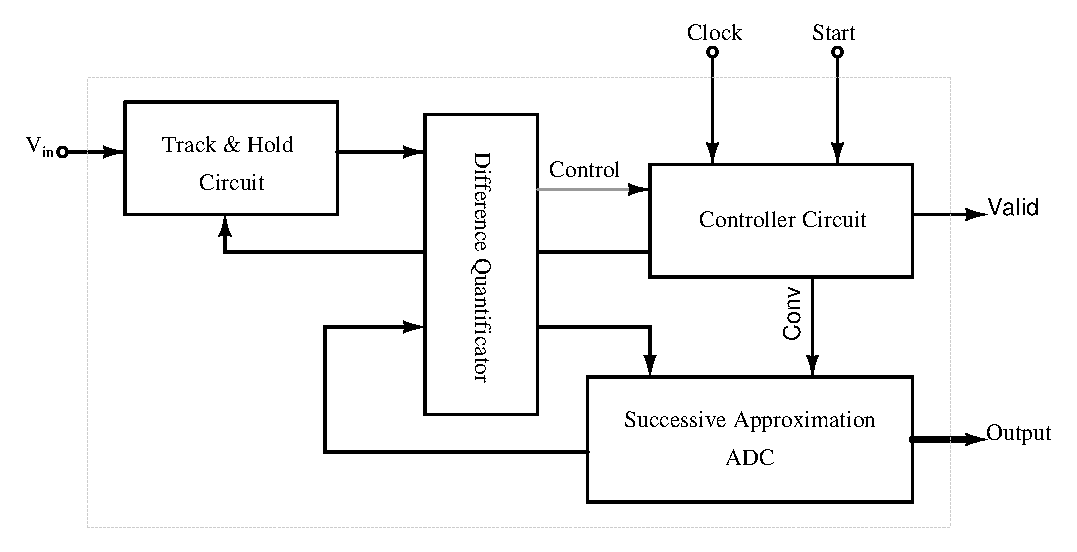
\includegraphics[scale=0.59]{./Figures/PADC.ps}
		\caption{Block Diagram of Proposed ADC}
		\label{fig:PADC}
	\end{center}
\end{figure}

\par
\hspace{0.6cm}  Controller circuit monitors the output of difference quantificator for a level crossing in the input analog signal. When the difference quantificator generates conversion signal the controller circuit generate all necessary control signals for the successive approximation ADC to convert the sampled analog signal into digital output, after completion of the conversion the analog output of the DAC is used to generate reference signal for the difference quantificator.

\par
\hspace{0.6cm} The controller circuit is also capable of loading an intial value in successive approximation register of successive approximation ADC at ever conversion process. By loading an intilligent value into successive approximation register it further decrease the number of comparisions which results in quick conversion process. Loading of intial value in successive approximation register depends on the previous ouput of the level crossing ADC and the direction in which input analog signal is traversing. Depending upon the application of level crossing ADC the contents of the successive approximation register are set from most significant bit (MSB) to least significant bit (LSB) or from LSB to MSB. A high speed counter is used to calculate the time difference between the present sample and the previous sample.

\par
\hspace{0.6cm} The proposed controller tracks the analog input in logarathmic fashion rather then linear fashion which is generally followed in conventional level crossing ADC's. At maximum the proposed level crossing ADC takes $2N$ clock cycles for complete the process in low frequency applications and $N$ clock cycles for high frequency applications. Where as in convetional  level crossing ADC's which use up-down counter will take $2^N$ clock cycles to complete the operation when the analog input changes from minimum to maximum value. Further the controller circuit can be programmed for low frequency applications in such a way that the maximum number of clock cycles required to convert input analog signal when changing from minimum to maximum can range in between $N$ to $2N$, where $N$ is the number of bits in level crossing ADC.\par


\section{Controller for high frequency applications}

\par
\hspace{1.2cm} In high frequency applications the input analog signal varies very rapidly. So, the bits in successive approximation register are set from the MSB to LSB. Some of the bits in the successive approximation register can be retained depending on the direction of the input analog signal traversing and the previous output of the level crossing ADC. The number of bits retained is same as the number of comparisions not needed to evaluate the present sampled analog signal which required to convert into digital output. The operation of controller circuit for high frequency applicatons is shown in Fig.~\ref{fig:HFA} as a flow chart for 8-bit hardwear resolution. \par


\par
\hspace{0.6cm} When the analog input signal is increasing then the present level crossing ADC output should be larger than the previous level crossing ADC output. So, all comparisons which results in present level crossing ADC output less than compared to previous level crossing ADC output can be eliminated. Similarly, when the analog input signal is decreasing then the present level crossing ADC output should be less then the previous level crossing ADC output. So, all coaprisons which results in present level crossing ADC output greater than compared to previous level crossing ADC Can be eliminated. The above situtions translated into the following process when setting the intial value into the successive approximation register.

\begin{figure}[H]
	\begin{center}
		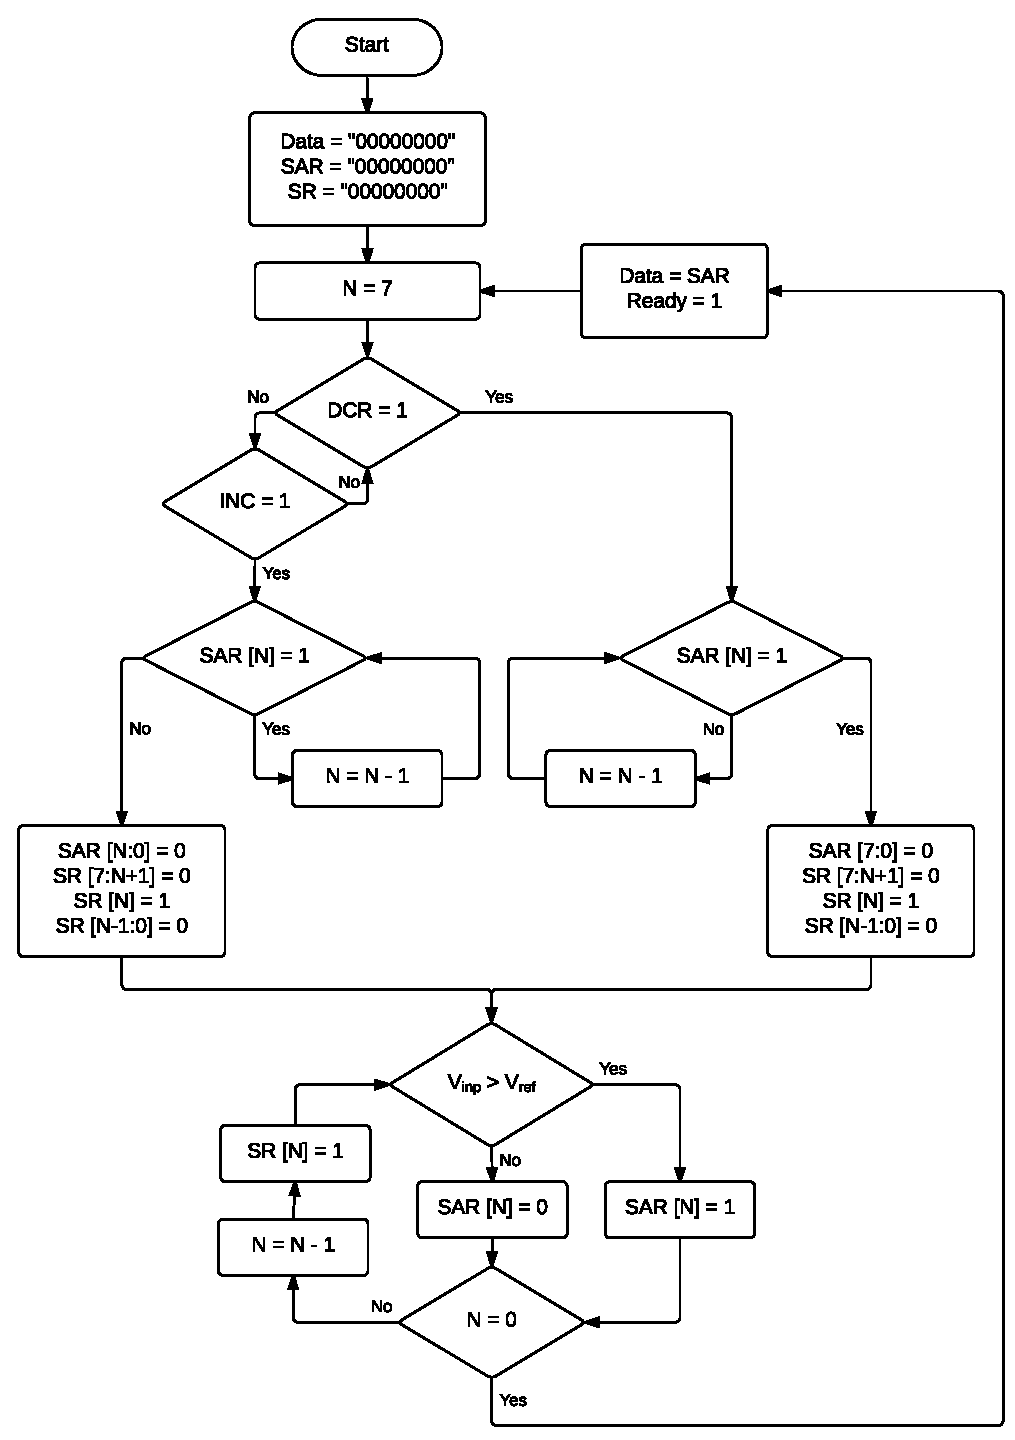
\includegraphics[width=10.1 cm, angle=360]{./Figures/HFA.ps}
		\caption{Controller operation for high frequency applications}
		\label{fig:HFA}
	\end{center}
\end{figure}

\par
\hspace{0.6cm} If the input analog signal is increasing the successive approximation register is assigned with all MS bits to '1' until first '0' and remaining bits are set to '0'. Shift Register is assigned with with all '0' except the first '0' in successive approximation register bit is set to '1'. If the input signal is decreasing the successive approximation register is assigned with all bits set to '0'. Shift Register is assigned with with all '0' except the first '1' in successive approximation register bit is set to '1'. Following examples demonstrates the situation for the proposed level crossing ADC to reduce the activity of the conversion circuit for high frequency applications. Fig.~\ref{fig:MHF} shows the Matlab result for reduction in activity with respect to the binary code for both the cases when the input analog signal is increasing and decreasing.

\par
\hspace{0.6cm}\textbf{Example 1}: When analog input is increasing if contents of successive approximation register are $11010110$, then value assigned to Shift Register is $00100000$ and value assigned to successive approximation register is $11000000$, which results reduction in two comparison states.

\begin{table}[h]		
	\begin{center}	
		\begin{tabular}{ c  c  c  c  c  c  c  c  c }
					Shift Reg  	& 0 & 0 & \textbf{1} & 0 & 0 & 0 & 0 & 0 \\
				   				&  &  & $\Uparrow$ & & & & & \\		
	 				\textbf{Output}   & \textbf{1} & \textbf{1} & \textbf{0} & 0 & 1 & 1 & 1 & 0 \\
				   				& $\Downarrow$ & $\Downarrow$ & & & & & & \\
					SA Reg     	& \textbf{1} & \textbf{1} & 0 & 0 & 0 & 0 & 0 & 0 \\			
		\end{tabular}
	\end{center}
\end{table}

\par
\hspace{0.6cm}\textbf{Example 2}: When analog input is decreasing if contents of successive approximation register are  $00010110$, then value assigned to Shift Register is $00010000$ and value assigned to successive approximation register is $00000000$, which results reduction in two comparison states.

\begin{table}[h]
\begin{center}	
		\begin{tabular}{ c  c  c  c  c  c  c  c  c }
					Shift Reg  	& 0 & 0 & 0 & 0 & \textbf{1} & 0 & 0 & 0 \\
				   				& &  &  &  &$\Uparrow$ & & & \\	
	 		 		\textbf{Output}   & \textbf{0} & \textbf{0} & \textbf{0} & \textbf{0} & \textbf{1} & 1 & 1 & 0 \\
				   				& $\Downarrow$ & $\Downarrow$ &  $\Downarrow$ &  $\Downarrow$ & & & & \\
					SA Reg     	& \textbf{0} & \textbf{0} & \textbf{0} & \textbf{0} & 0 & 0 & 0 & 0 \\
			
		\end{tabular}
	\end{center}
\end{table}

\begin{figure}[H]
	\begin{center}
		\includegraphics[scale=0.4]{./Figures/FAST.eps}
		\caption{Reduction in activity with digital code}
		\label{fig:MHF}
	\end{center}
\end{figure}



\section{Controller for low frequency applications}

\par
\hspace{1.2cm} In low frequency applications the input analog signal varies slowly. So, the bits in successive approximation register are set from the LSB to MSB. Some of the bits in the successive approximation register can be retained depending on the direction of the input analog signal traversing and the previous output of the level crossing ADC. The operation of controller for low frequency applicatons is shown in Fig.~\ref{fig:LFA} as a flow chart for 8-bit hardwear resolution. \par

\begin{figure}[H]
	\begin{center}
		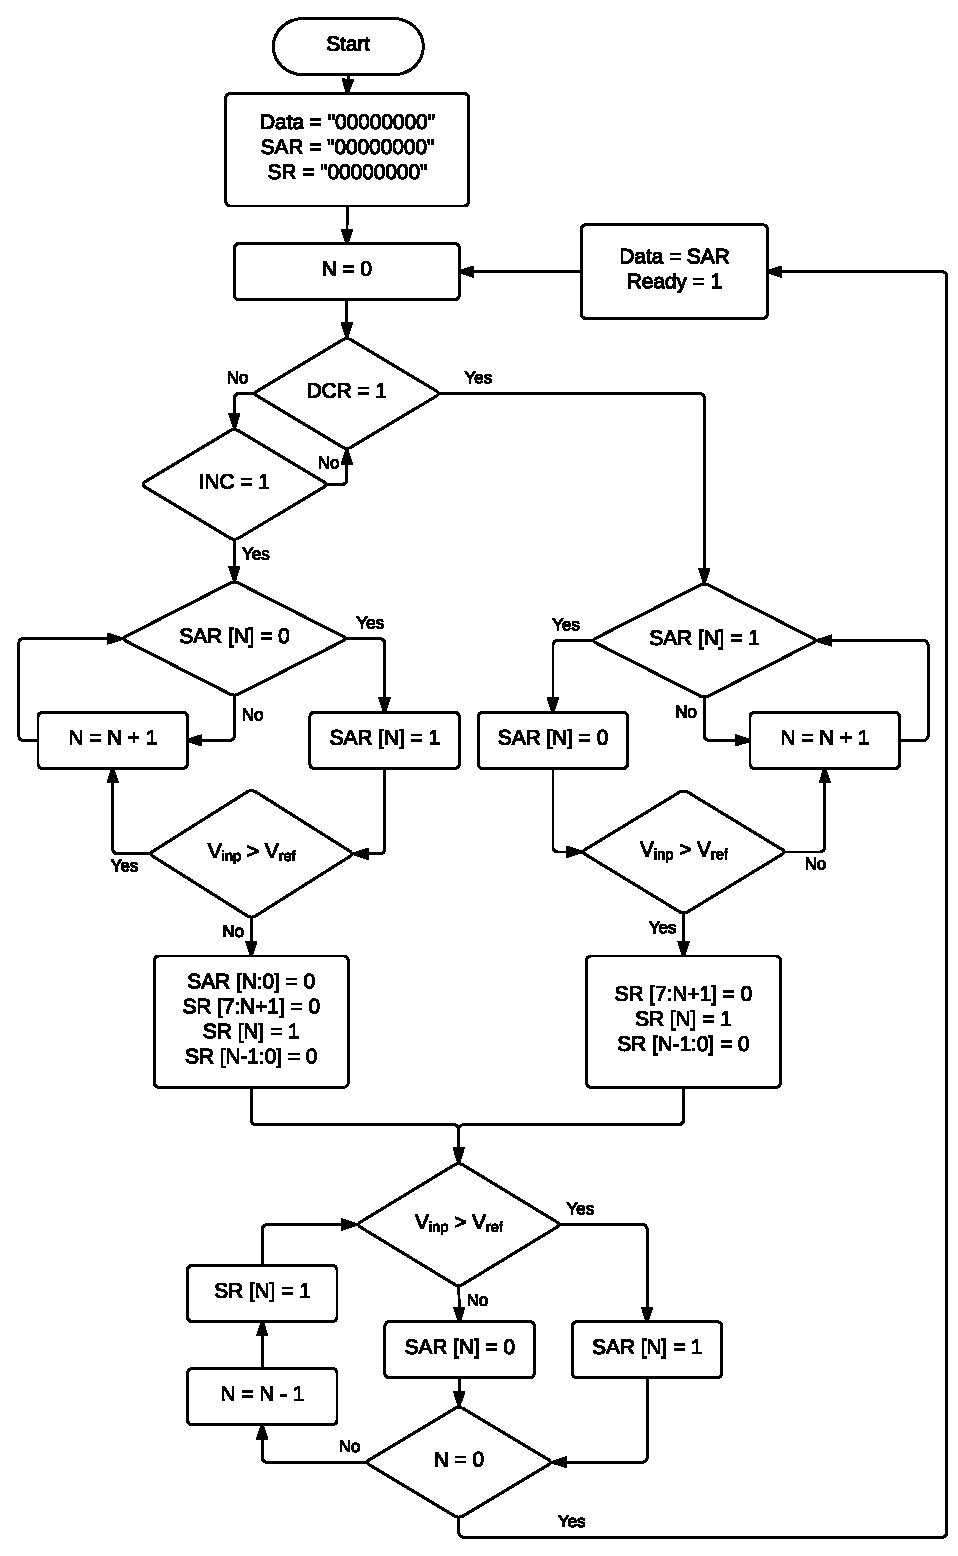
\includegraphics[width=9.8 cm, angle=360]{./Figures/LFA.ps}
		\caption{Controller operation for low frequency applications}
		\label{fig:LFA}
	\end{center}
\end{figure}

\par
\hspace{0.6cm} The controller circuit works in two phases for both the cases when input analog signal increasing or decreasing. In first phase it checks for the vilation of the obtained condition and in the second phase it estimates the exact value of the sampled analog signal. In first phase when the input analog signal is increasing then the '0's from LSB will be converted into '1's one by one and checking whether the resulting signal is greater than input analog signal. until the case is achieved all bits from LSB to MSB are converted to 1's. When the condition is reached all the MSB bits are copied as they are upto the current bit and all remaing bits are assigned with zeros in successive approximation register. The shift register is loaded with all zeros except the bit when the condition is achieved is made one and then normal sucessive approximation conversion process is folled. 

\par
\hspace{0.6cm} Similarly, when the input analog signal is decreasing then the 1's from LSB will be converted into 0's one by one and checking whether the resulting signal is less than input analog signal. Until this condition is achieved all bits from LSB to MSB are converted to 0's. When the condition is reached all the MSB bits are copied as they are upto the curren bit and all remaining bits are assigned with zeros in successive approximation register. the shift register is loaded with all zeros except the bit when the condition is achieved is made one and then normal successive approximation process is followed to finad the exact value of the sampled analog signal.   

\par
\hspace{0.6cm} Following examples demonstrates the situation for the proposed level crossing ADC to reduce the activity of the conversion circuit for high frequency applications. Fig.~\ref{fig:MHF} shows the Matlab result for reduction in activity with respect to the binary code for both the cases when the input analog signal is increasing and decreasing.

\begin{figure}[H]
	\begin{center}
		\includegraphics[scale=0.4]{./Figures/SLOW.eps}
		\caption{Reduction in activity with digital code}
		\label{fig:MLF}
	\end{center}
\end{figure}



\chapter{Building Blocks}

\section{Sample and Hold}
\begin{figure}[H]
	\begin{center}
		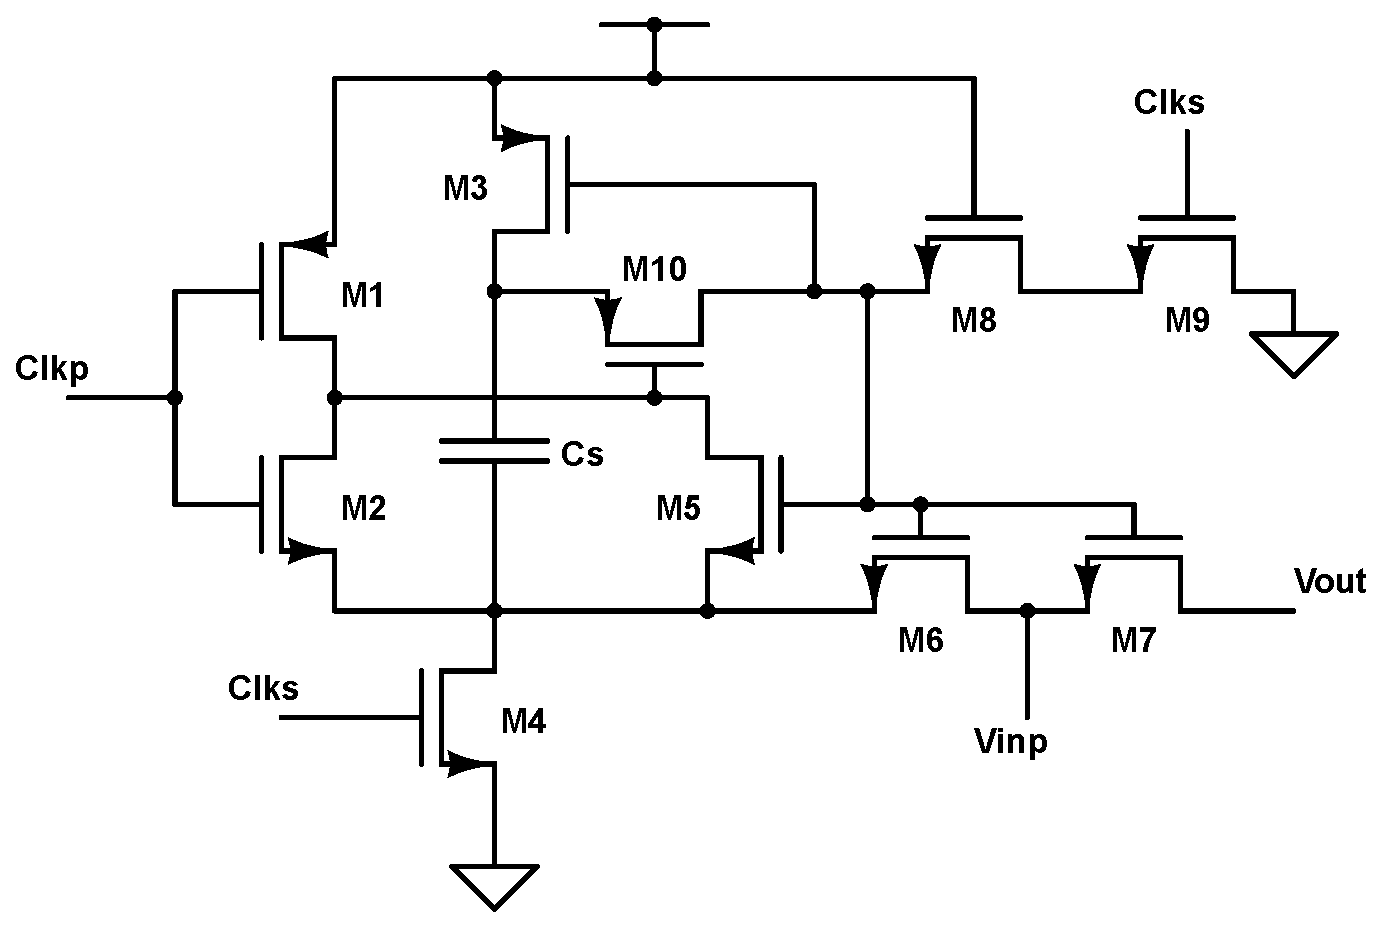
\includegraphics[scale=0.4]{./Figures/BSS.eps}
		\caption{Circuit diagram of sample and hold}
		\label{fig:BSS}
	\end{center}
\end{figure}

\section{Clcked Comparator}
\begin{figure}[H]
	\begin{center}
		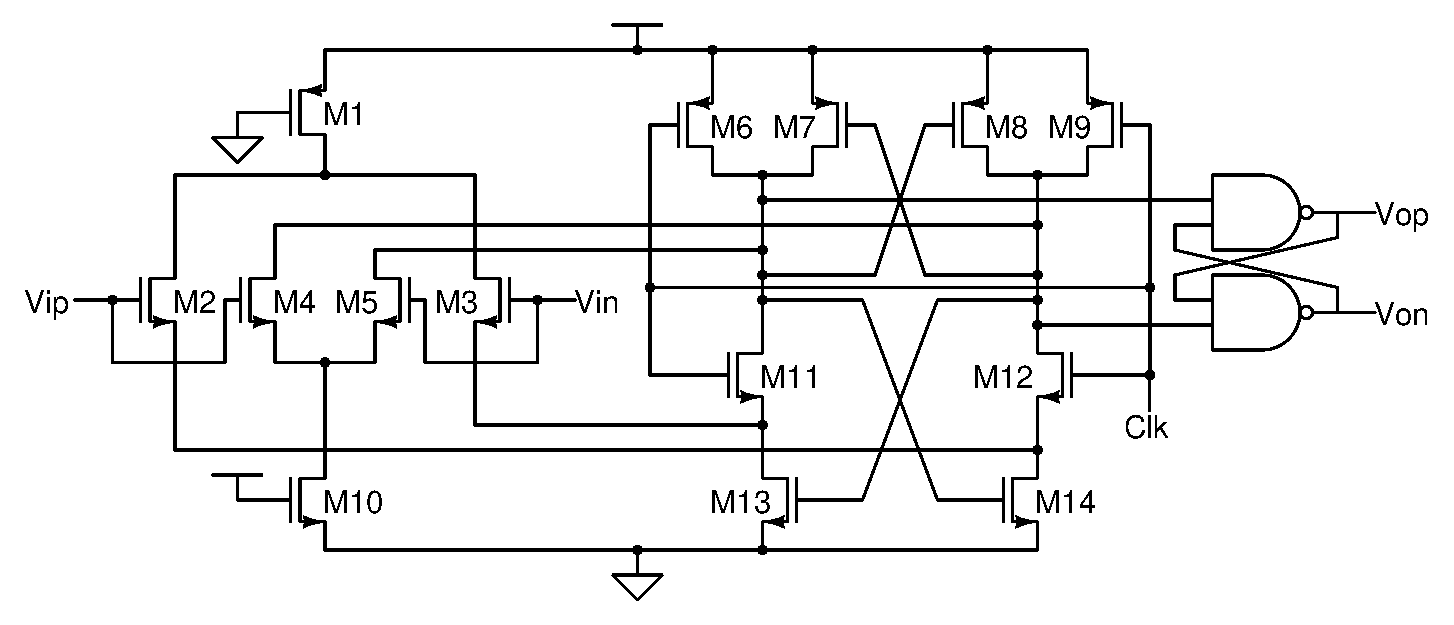
\includegraphics[scale=0.6]{./Figures/CMP.eps}
		\caption{Circuit diagram of clocked comparator}
		\label{fig:CMP}
	\end{center}
\end{figure}

\section{Proposed Digital-to-Analog converter}
\begin{figure}[H]
	\begin{center}
		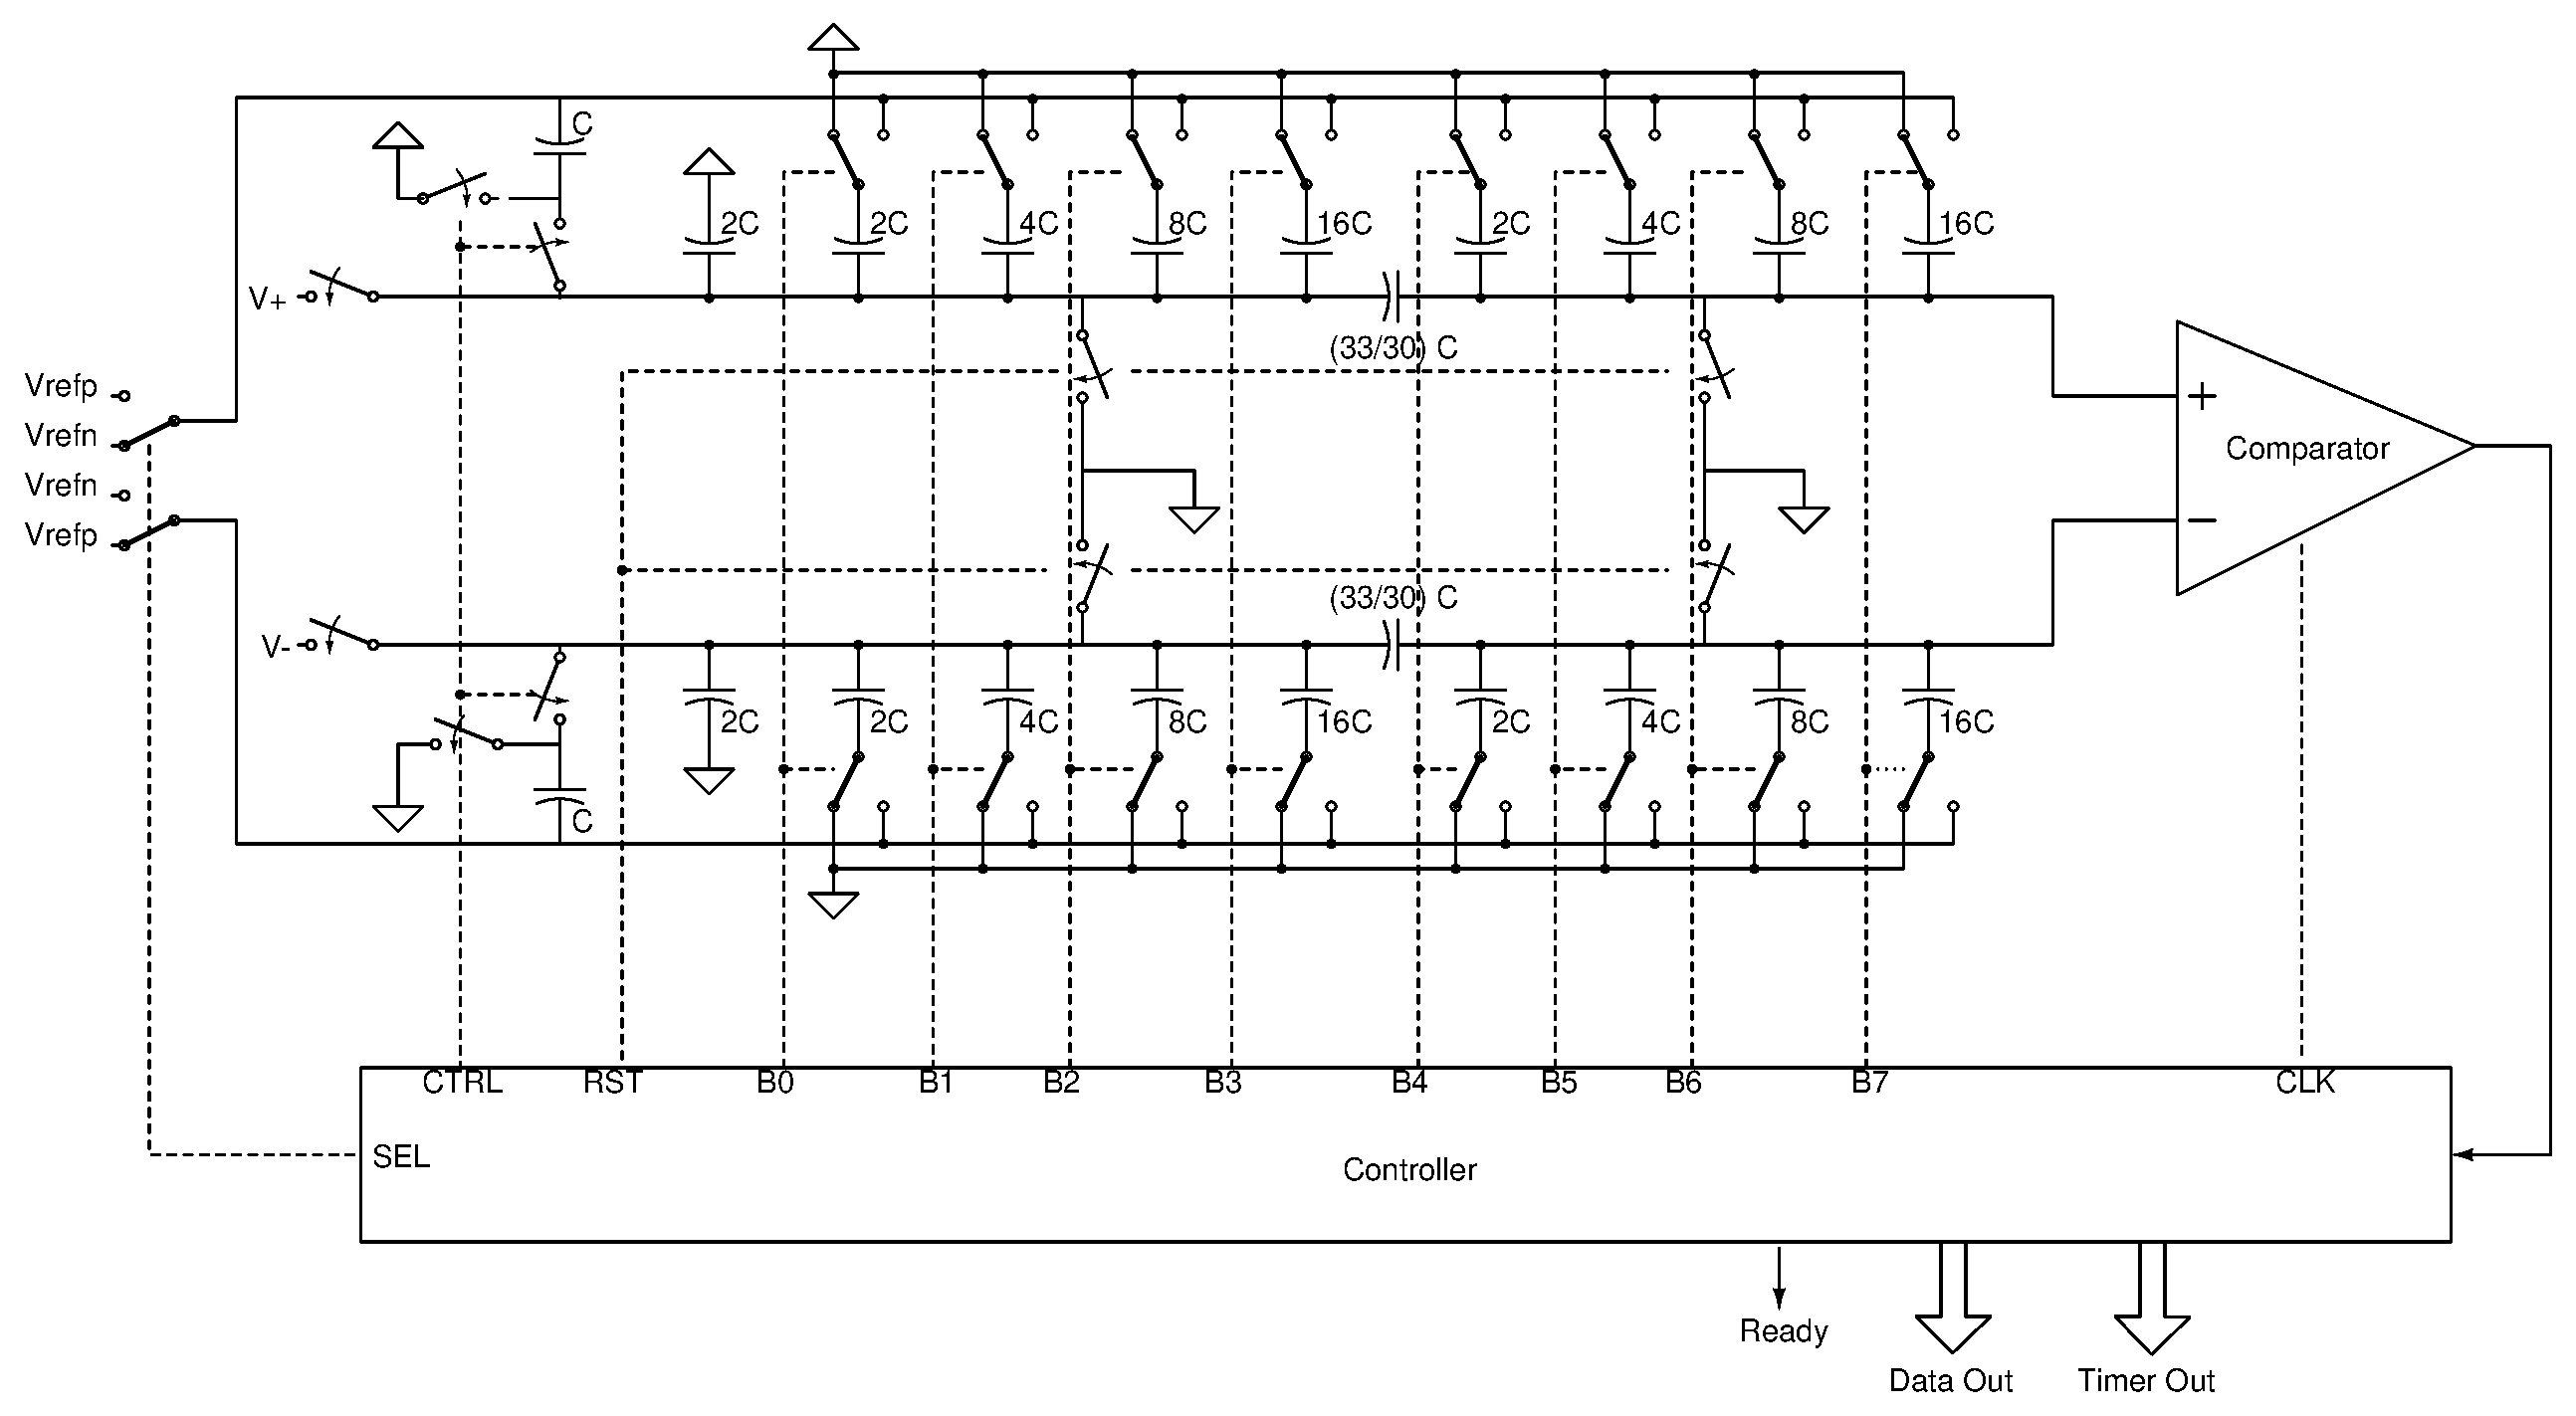
\includegraphics[scale=0.4, angle=360]{./Figures/ADC.eps}
		\caption{Block diagram of proposed ADC}
		\label{fig:CMP}
	\end{center}
\end{figure}



\chapter{Conclusion and Future Work}


\section{Conclusion}

\par
\hspace{1.2cm} In this report, a 8-bit A to D converter is proposed , which is designed in CMOS UMC 180 nanometer technology, with semi-custom design by using Farady design kit. The proposed successive approximation A to D converter can reduce power by reducing the activity of the circuit. It is a hybrid of both level cross sampling and Nyquist sampling. The sampling takes place in track and hold circuit as per Nyquist sampling but the conversion process is initiated by level cross sampling method. Further number of conversion cycles in proposed successive approximation A to D converter can be reduced by adjusting the preset data to the comparator array.


\section{Future Work}

\par
\hspace{1.2cm} Future work includes completion of proposed successive A to D converter and send it for fabrication and testing of it. The activity of the circuit depends on the resolution of analog to digital converter, so a variable resolution analog to digital converter will reduce more power, when the low resolution is sufficient for the application, to implement this the difference quantificator has the option to change it's window size by external input so that the conversion process initiated by the difference quantificator will be reduced. 




\renewcommand\bibname{References}
\bibliographystyle{IEEE}
\bibliography{References}
\addcontentsline{toc}{chapter}{References}
%\addcontentsline{toc}{chapter}{References}
\begin{thebibliography}{10}


\bibitem{1P}
E. Allier, J. Goulier, G. Sicard, A. Dezzani, E. Andre and M. Renaudin, "A 120nm low power asynchronous ADC," \emph {International Symposium on Low Power Electronics and Design}, 2005.

\bibitem{2P}
F. Akopyan, R. Manohar, and A. B. Apsel, "A level-crossing flash asynchronous analog-to-digital converter," \emph {International Symposium on Asynchronous Circuits and Systems}, 2006.

\bibitem{7P}
E. Allier, G. Sicard, L. Fesquet and M. Renaudin, "Asynchronous level crossing analog to digital converters," \emph {Elsevier Journal of the International Measurement Confederation}, 2005.

\bibitem{8P}
A. Fayed and M. Ismail, "A High Speed, Low Voltage CMOS Offset Comparator," \emph {Analog Integrated Circuits and Signal Processing}, 2003.

\bibitem{9P}
 Daegyu Lee, Jincheol Yoo, Kyusun Choi and J. Ghaznavi, "Fat tree encoder design for ultra-high speed flash A/D converters," \emph { Midwest Symposium on Circuits and Systems}, 2002.


\bibitem{3P}
R. Agarwal, M. Trakimas and S. Sonkusale, "Adaptive asynchronous analog to digital conversion for compressed biomedical sensing," \emph {IEEE Conference on Biomedical Circuits and Systems}, 2009.

\bibitem{4P}
M. Trakimas, S. Sonkusale,  "A 0.8 V asynchronous ADC for energy constrained sensing applications," \emph {IEEE Conference on Custom Integrated Circuits Conference}, 2008.

\bibitem{5P}
S. W. Michael and R. W. Brodersen "A 6-bit 600-MS/s 5.3-mW Asynchronous ADC in 0.13$\mu$m CMOS," \emph {IEEE Journal of Solid-State Circuits}, 2006.

\bibitem{6P}
Ying-Zu Lin, Soon-Jyh Chang, Yen-Ting Liu, Chun-Cheng Liu and Guan-Ying Huang, "An Asynchronous Binary-Search ADC Architecture With a Reduced Comparator Count," \emph {IEEE Transactions on Circuits and Systems}, 2010.

\bibitem{1L}
B. Murmann, "ADC Performance Survey 1997-2010," [Online]. Available: $http://www.stanford.edu/~murmann/adcsurvey.html$.

\end{thebibliography}

\end{document}
